\documentclass[11pt]{jarticle}

\usepackage[dvipdfmx]{graphicx}
\newcommand{\setPicture}[1]{\includegraphics[width=1\linewidth]{chapters/picture/#1}}
\usepackage{sty/fancyheadings}
\usepackage{sty/sotsuron2009}
\usepackage{here}
\usepackage{ascmac}
\usepackage[subrefformat=parens]{subcaption}
\usepackage{here}
\usepackage{cite}
\usepackage{amsmath}
\pagestyle{empty}
\usepackage{bm}
\usepackage{comment}
\linesparpage{40}
%\makeatletter
%\renewcommand{\theequation}{
%\thesection.\arabic{equation}}
%\@addtoreset{equation}{section}
%\makeatother
\pagestyle{fancy}

\newcommand{\argmin}{\mathop{\rm arg~min}\limits}
\setcounter{topnumber}{5}
\setcounter{bottomnumber}{5}
\setcounter{totalnumber}{10}
\renewcommand{\textfraction}{0.0}
\renewcommand{\topfraction}{1.0}

\newcommand{\Section}[1]{\section*{#1}
\addcontentsline{toc}{section}{#1}}
\newcommand{\Subsection}[1]{\section*{#1}
\addcontentsline{toc}{subsection}{#1}}
\renewcommand{\refname}{}


\begin{document}

\begin{comment}
\title{
 \LARGE
 % 卒論和文タイトル
 \\ \\
 \large
 % 卒論英文タイトル
}

\author{
 研究者 高専 太郎\\
 指導教員 中西 大輔\\ \\
 松江工業高等専門学校\\
 電子制御工学科\\ \\
}

\date{平成29年2月13日}

\maketitle
\end{comment}

\thispagestyle{empty}
\newpage
\section*{概要}
水中の推進システムにはスクリュープロペラを用いた推進方法や魚を模したロボットによる尾びれ推進などがあげられる.スクリュープロペラは水上,水中における推進性能が高く,
船舶などに広く用いられている.しかし,生態系調査の面で考えると,スクリュープロペラは周辺環境に影響を与え,調査に適しているとは言えない.その一方で尾びれ推進は周辺環境に影響を与えることがなく,尚且つ加速性・旋回性に優れているため障害物を避けながら目的の地点まで速やかな移動を可能にする.以上のことから水害などの災害支援,水中生物の
生態系調査の面で魚型ロボットの開発は注目されている.そこで我々の研究室ではこれまで様々な魚型ロボットを開発してきた.特に昨年度は魚らしくしなやかな動きを可能にするワイヤ駆動
式の魚ロボットと,完全防水可能かつ魚らしい流線形のボディを有する柔軟外皮装着型の魚ロボットの開発に成功した.しかし,昨年度の先行研究には次のような課題があった.ワイヤ駆動式の
魚ロボットには骨格リンク間にできる隙間に水が入り込み,体全体を使って水をかけないといった課題が,柔軟外皮装着型のロボットには骨格リンクの動きに外皮が追従せず,十分な遊泳性能を
得られなかったという課題があった.そこで本研究ではワイヤ駆動式の魚ロボットに柔軟外皮を装着することによって,魚らしいしなやかな動きを可能にし,かつ骨格リンクの動きに外皮が追従
できるようにすることで十分な遊泳性能を発揮できる魚ロボットを開発した.また,外皮あり・なしそれぞれで直進遊泳実験を行い,外皮による遊泳性能に与える影響について検証を行った.遊
泳実験の結果,外皮を装着することによって遊泳速度が向上することがわかった.速度が向上した要因としては,ロボットのボディが外皮を装着することによって流線形になったことが考えられ
る.したがって流線形のボディを備えることは,遊泳速度を向上させるのに非常に有効であると考えられる.
\newpage
\section*{Abstract}
In underwater propulsion systems, methods such as using screw propellers and fish-like robots with tail fin propulsion are commonly mentioned. Screw propellers 
have high propulsion performance both on the water surface and underwater, and are widely used in ships and other vessels. However, from the perspective of ecosystem 
surveys, screw propellers are not ideal, as they can impact the surrounding environment and are not suitable for surveys. On the other hand, tail fin propulsion 
does not affect the surrounding environment, and its excellent acceleration and maneuverability enable swift movement to a target location while avoiding obstacles. 
For these reasons, the development of fish-like robots has attracted attention for applications in disaster response, such as in the case of flooding, and for aquatic 
ecosystem surveys.
In our laboratory, we have developed various types of fish-like robots. In particular, last year we succeeded in developing a wire-driven fish robot that enables 
flexible movements similar to a real fish, as well as a soft-skin fish robot with a streamlined body and complete waterproofing. However, there were some challenges 
in last year's research. The wire-driven fish robot faced the issue of water entering the gaps between the skeletal links, which prevented efficient water management 
across the entire body. The soft-skin robot encountered the problem that the skin did not follow the movements of the skeletal links, leading to insufficient swimming 
performance.
Therefore, in this study, we developed a fish robot by attaching a soft skin to the wire-driven robot, enabling flexible, fish-like movements while allowing the skin 
to follow the movement of the skeletal links. This development ensures sufficient swimming performance. Additionally, we conducted swimming experiments with and without 
the soft skin to investigate the impact of the soft skin on swimming performance. The results of these experiments showed that the swimming speed increased when the soft 
skin was attached. The increase in speed is believed to be due to the streamlined body shape achieved by the soft skin. Hence, it can be concluded that having a streamlined 
body is highly effective in improving swimming speed.
        % 概要

\thispagestyle{empty}
\newpage
\tableofcontents
\thispagestyle{empty}

%章ごとに呼び出し

\newpage
\setcounter{page}{1}
\section{緒言}
水中の推進システムにはスクリュープロペラを用いた推進方法や魚を模したロボットによる尾びれ推進などがあげられる\cite{ichi}.スクリュープロペラは水上,水中における推進性能が高く,
船舶などに広く用いられている.しかし,生態系調査の面で考えると,スクリュープロペラは周辺の植物や水中動物などを巻き込んで水中の環境に影響を与え,騒音によって周辺生物を
驚かせるなど,調査に適しているとは言えない.その一方で尾びれ推進は周辺生物を巻き込むなど環境に影響を与えにくく,尚且つ加速性・旋回性に優れているため障害物を避けながら
目的の地点まで高機動な遊泳を可能にする.以上のことから水害などの災害支援,水中生物の生態系調査の面で魚型ロボットの開発は注目されている\cite{ni}\cite{san}.

そこで我々の研究室ではこれまで様々な魚型ロボットを開発してきた.駆動機構として弾性体を用いた飛び移り座屈機構を採用した魚ロボット\cite{yon}\cite{go}や,それに加えて屈曲可能な胴体
構造を有する魚ロボット\cite{roku,nana,hachi}の開発に成功してきた.さらに昨年度卒業研究では駆動機構としてワイヤ駆動方式を用いたより魚らしい形状を持つ魚ロボットの開発に成功し,
魚のように胴体を屈曲させてしなやかに遊泳を行うことができた.しかし,これらの魚ロボットには弾性体に追従する骨格リンクの隙間に水が入り込み,結果的に弾性体のみで水をかいてしまい,体全体でかく
ことができていないという課題があった.

一方で同じく昨年度卒業研究(先行研究\cite{kyu})ではこの課題を解決するために,胴体部全体をシリコン製の柔軟外皮で覆った魚型ロボットの開発が行われた.柔軟外皮は魚らしい流線型のフォルムの実現のみならず,従来のOリングを
用いた手法よりも容易かつ確実性の高い防水性能を実現した.しかし,遊泳に関しては骨格リンクの動きに柔軟外皮が追従せず,胴体部を振って泳ぐことはできなかった.そのため遊泳速度が大きく低下し,柔軟
外皮が遊泳速度に対してどのように影響を与えるのか検証することができなかった.

そこで本研究では,しなやかな遊泳が可能なワイヤ駆動方式と,流線形の胴体フォルムを実現可能な柔軟外皮を組み合わせた魚型ロボットを開発する.ロボットはアジのスキャンデータを基に作成し,アジ型遊泳の定義\cite{juu}のもとに,
胴体後ろ半分を屈曲させることで遊泳を行う.そして柔軟外皮あり・なしで直進遊泳実験を行い,柔軟外皮が遊泳性能に与える影響について検証・考察を行う.
    % 緒言
\newpage
\section{先行研究}
本章では,本研究で開発したロボットのベースとなった機体を先行研究を用いて述べ,それぞれの実験結果とそこから得られた知見をまとめる.

\subsection{柔軟外皮装着型魚ロボット}
先行研究\cite{kyu}で開発された機体を図\ref{fig:robot_sen}\cite{kyu}に,構造を図\ref{fig:kouzou_sen}\cite{kyu}に示す.先行研究\cite{kyu}ではハマチをモデルにしてロボットを作製していた.
図\ref{fig:migaihi_sen}は魚型ロボットに柔軟外皮を取り付けたものであり,水中に沈めること及び水中での姿勢維持を目的として,柔軟外皮を固定する防水リングにおもりが取り付けてある.おもり
の重さは頭部と尾びれ部分でそれぞれ296 g,150 gである.本機体は全長477 mm,重さ1080 g,おもりを含めた重さが1526 gとなっている.本機体は頭部と胴体部の大きく二つに分けることができる.

\begin{figure}[htbp]
    \centering
    \begin{tabular}{cc}
     \begin{minipage}[b]{0.45\linewidth}
        \centering
        \setPicture{zenrarobot.jpg}
        \subcaption{外皮未装着時}
        \label{fig:gaihi_sen}
     \end{minipage}
     \hspace{0.05\linewidth}
     \begin{minipage}[b]{0.45\linewidth}
        \centering
        \setPicture{fishrobot.jpg}
        \subcaption{外皮装着時}
        \label{fig:migaihi_sen}
     \end{minipage}
    \end{tabular}
    \caption{柔軟外皮装着型の魚ロボット\cite{kyu}}
    \label{fig:robot_sen}
\end{figure}
\begin{figure}[b]
    \centering
    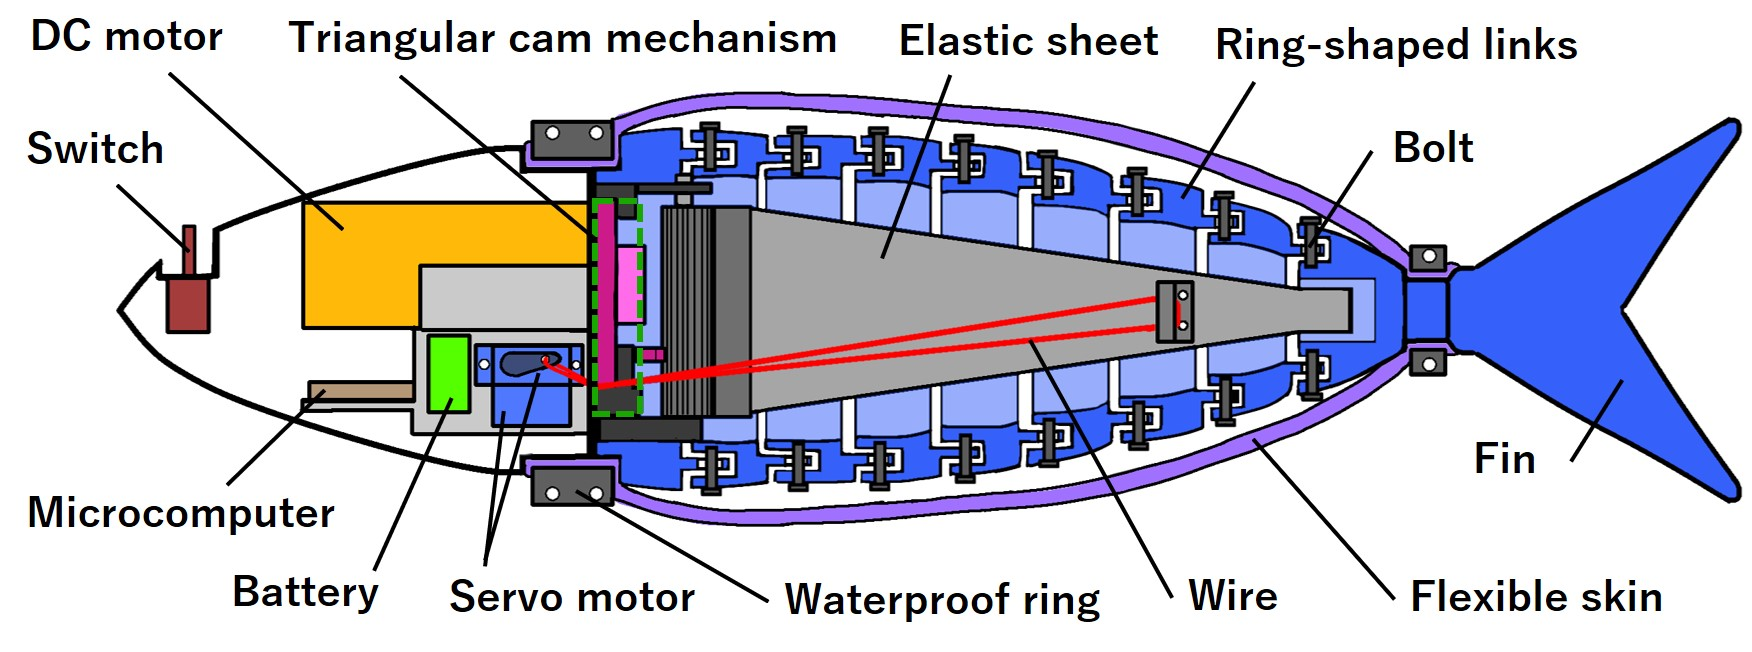
\includegraphics[width=1\linewidth]{chapters/picture/mosikizu.jpg}
    \caption{ロボットの構造\cite{kyu}}
    \label{fig:kouzou_sen}
\end{figure}

\subsubsection{頭部}
本機体の頭部には,DC モータ( タミヤ社,AO-8033),サーボモータ(Tower Pro 社,MG92B)二つ,マイコン(M5Stack Technology 社,M5STACK-K051),モータ用Lipo バッ
テリ(Hyperion 社,G5 50Cmax 7.4 V-240 mAh),マイコン用Lipo バッテリ(DATA POWERTECHNOLOGY 社,DTP502535),スイッチが入っている.モータは頭部に収まるものの中
でなるべくトルクの強いものが用いられている.また,上に挙げたスイッチ以外の部品はすべて頭部の外殻ではなく内側のふたに取り付けられている.

\begin{figure}[t]
    \centering
     \begin{minipage}[b]{0.45\linewidth}
        \centering
        \setPicture{zakutu1.png}
        \caption{飛び移り座屈発生機構の模式図\cite{kyu}}
        \label{fig:zakutu1_sen}
     \end{minipage}
     \begin{minipage}[b]{0.35\linewidth}
        \centering
        \setPicture{zakutu2.png}
        \caption{たわみ長さの定義\cite{kyu}}
        \label{fig:zakutu2_sen}
     \end{minipage}
     \begin{minipage}[b]{0.15\linewidth}
        \centering
        \setPicture{link.png}
        \caption{関節の構造\cite{kyu}}
        \label{fig:kansetu}
     \end{minipage}
\end{figure}

\subsubsection{胴体部}
まず,先行研究\cite{kyu}で駆動機構として用いられた飛び移り座屈について記す.飛び移り座屈とは,弾性を有する柔軟体の変形によって発生する連続的な現象であり,
瞬間的に大きな力を発生させることができる.先行研究ではサーボモータを用いて弾性体をたわませ,DCモータを用いて弾性体を変形させることで飛び移り座屈を
発生させている.ここで実験に用いる語句とパラメータを定義する.図\ref{fig:zakutu1_sen}に飛び移り座屈発生機構の模式図を示す.弾性体の自然長を$l$,弾性体をたわませた際の軸間
距離を$L$,弾性体がどの程度たわんでいるかを示すたわみ長さを$d$として,たわみ長さを$d=l−L$と定義する.

次に胴体部について,胴体部は屈曲可能な8関節9リンク構造になっており,リンクの接続部は図\ref{fig:kansetu}のようにベアリング(内径3 mm)とボルト(M2)で接続されている.
また,すべてのリンクで合計$90\:^\circ$曲げるため一関節あたり$11.25\:^\circ$曲がるよう設計されている.$90\:^\circ$という値は,実際のハマチの動く様子から決定している.
なお,各リンクには機体を水中に沈めるために板おもり(22 g)を合計10 枚張り付けてある.次に,飛び移り座屈に用いる弾性体について記す.ここでの弾性体とは外力により曲がる薄
い板のことを指す.先行研究では0.2 mm厚のステンレス(岩田製作所,SUS02)に加え,弾性を強めるために1 mm厚のポリプロピレン(セイワ・プロ社,23-589)を貼り合わせたものを使用している.

\subsection{遊泳実験}
\subsubsection{実験条件}
直進遊泳をさせるため,サーボモータを$90\:^\circ$回し,たわみ長さを10 mmに固定した.その上でDCモータに印加する電圧を1.5 V,2.0 V,2.5 Vに変化させて遊泳を行っ
た.また,機体内部に防水シールを貼り,遊泳時においても防水ができているか確認する.



\subsubsection{実験結果}
印加電圧1.5 V時の遊泳の様子を図\ref{fig:swim_sen}に示す.遊泳には成功したが,遊泳の軌道が少し曲がってしまっていることがわかる.また,印加電圧と遊泳速度の関係を図\ref{fig:speed}に示す.
電圧が大きくなるにつれて,遊泳速度も大きくなっていることがわかる.本機体の最高遊泳速度は印加電圧2.5 V時の43 mm/sであった.
直進遊泳をするはずが少し曲がってしまったことについて,これは,弾性体をたわませる二つの糸の長さが異なることが原因として考えられる.弾性体をたわませ
る力が左右で違ったことにより飛び移り座屈で発生する力にも左右で差が出てしまうので,結果曲がってしまったと考えられる.
次に遊泳速度が遅い原因として2 つ考えられる.1 つ目はたわみ長さが小さかったことである.たわみ長さや尾びれの振れ角が大きい程飛び移り座屈を発生させたときに放出する
力は大きくなるが,飛び移り座屈を発生させるために必要な力も大きくなる.また2 つ目の原因として,外皮とリンクの間に余分な隙間があったため,リンクの動きを外皮に伝えることができな
かったということが考えられる.
\begin{figure}[htbp]
    \centering
    \begin{minipage}[b]{0.5\linewidth}
        \centering
        \setPicture{swim.png}
        \caption{遊泳実験の様子\cite{kyu}}
        \label{fig:swim_sen}  
    \end{minipage}
    \hspace{0.05\linewidth}
    \begin{minipage}[b]{0.4\linewidth}
        \centering
        \setPicture{speed.eps}
        \caption{印加電圧と遊泳速度の関係\cite{kyu}}
        \label{fig:speed}  
    \end{minipage} 
\end{figure}
\begin{figure}[b]
    \centering
    \begin{tabular}{ccc}
        \begin{minipage}[b]{0.3\linewidth}
            \centering
            \setPicture{aka.png}
            \subcaption{赤く染まった防水シール}
            \label{fig:aka_sen}
        \end{minipage}
        \begin{minipage}[b]{0.3\linewidth}
            \centering
            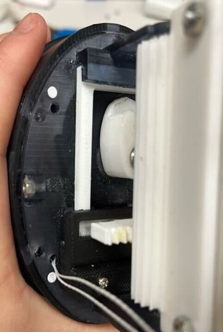
\includegraphics[width=0.6\linewidth]{chapters/picture/siro_naka.png}
            \subcaption{機体内部の防水シール}
            \label{fig:naka_sen}
        \end{minipage}
        \begin{minipage}[b]{0.3\linewidth}
            \centering
            \setPicture{siro_obire.png}
            \subcaption{尾びれ側の防水シール}
            \label{fig:obire_sen}
        \end{minipage}
    \end{tabular}
    \caption{遊泳実験後の防水シールの様子\cite{kyu}}
    \label{fig:bousui_sen}
\end{figure}
遊泳実験を行った後機体を開けてみると,防水シールはわずかに染まった一か所を除いてすべて白いままであった(図\ref{fig:bousui_sen}).このことから,機体内部の防水に成功したことが分かる.

\subsection{得られた知見}
先行研究では柔軟外皮を開発し,柔軟外皮を用いての完全防水に成功した.しかし,柔軟外皮と骨格リンクに隙間ができてしまい,リンクの動きに柔軟外皮を追従させることができなかった.柔軟外皮をリンクに密着
させる,または柔軟外皮とリンクを追従させるための構造を開発することによってリンクの動きを柔軟外皮に伝えることが可能だと考えられる.また,柔軟外皮を用いて胴体部に防水を行っていたため,胴体が浮袋に
なり重りを多く付ける必要があった.これについては胴体部を柔軟外皮で包んだ上で中に水を入れて浸水させることで,遊泳姿勢を重りを使わずに安定させることができると考える.            % 本文
\newpage
\section{柔軟外皮を備えたワイヤ駆動式魚ロボットの開発}
前章で述べたように,先行研究\cite{kyu}では屈曲可能な胴体を持ち,柔軟外皮を装着して完全防水を可能にした魚ロボットの開発に成功した.しかし,リンクと外皮に隙間ができてしまい,
リンクの動きを外皮にうまく伝えることができなかった.そこで本研究では魚らしいしなやかな動きを可能にするワイヤ駆動式の魚ロボットをベースにリンクに外皮を追従させ,尾びれのみならず
胴体部まで振って泳ぐことが可能なロボットの開発を目指す.本章ではその予備的な開発として,昨年度卒業研究を参考に外皮を持たないワイヤ駆動式魚型ロボットを開発し,柔軟外皮をどのよう
に組み合わせるべきかなどについて検討を行う.
\subsection{ワイヤ駆動式魚型ロボットの動作原理}
昨年度卒業研究で提案され,本研究でも採用したワイヤ駆動の動作原理を記す.ロボット前方にはプーリを取り付けたサーボモータを配置し,胴体部には弾性体とそれに固定した骨格リンクを配置する.
ワイヤはプーリーから骨格リンクに設けられた穴を通って尾びれ付け根まで伸びており,プーリーを回してワイヤを巻き取ることによって弾性体が曲がり,胴体部を屈曲させることができる.それを左
右に繰り返すことで遊泳を可能にする(図\ref{fig:waiyakudou}).

\begin{figure}[b]
   \centering
   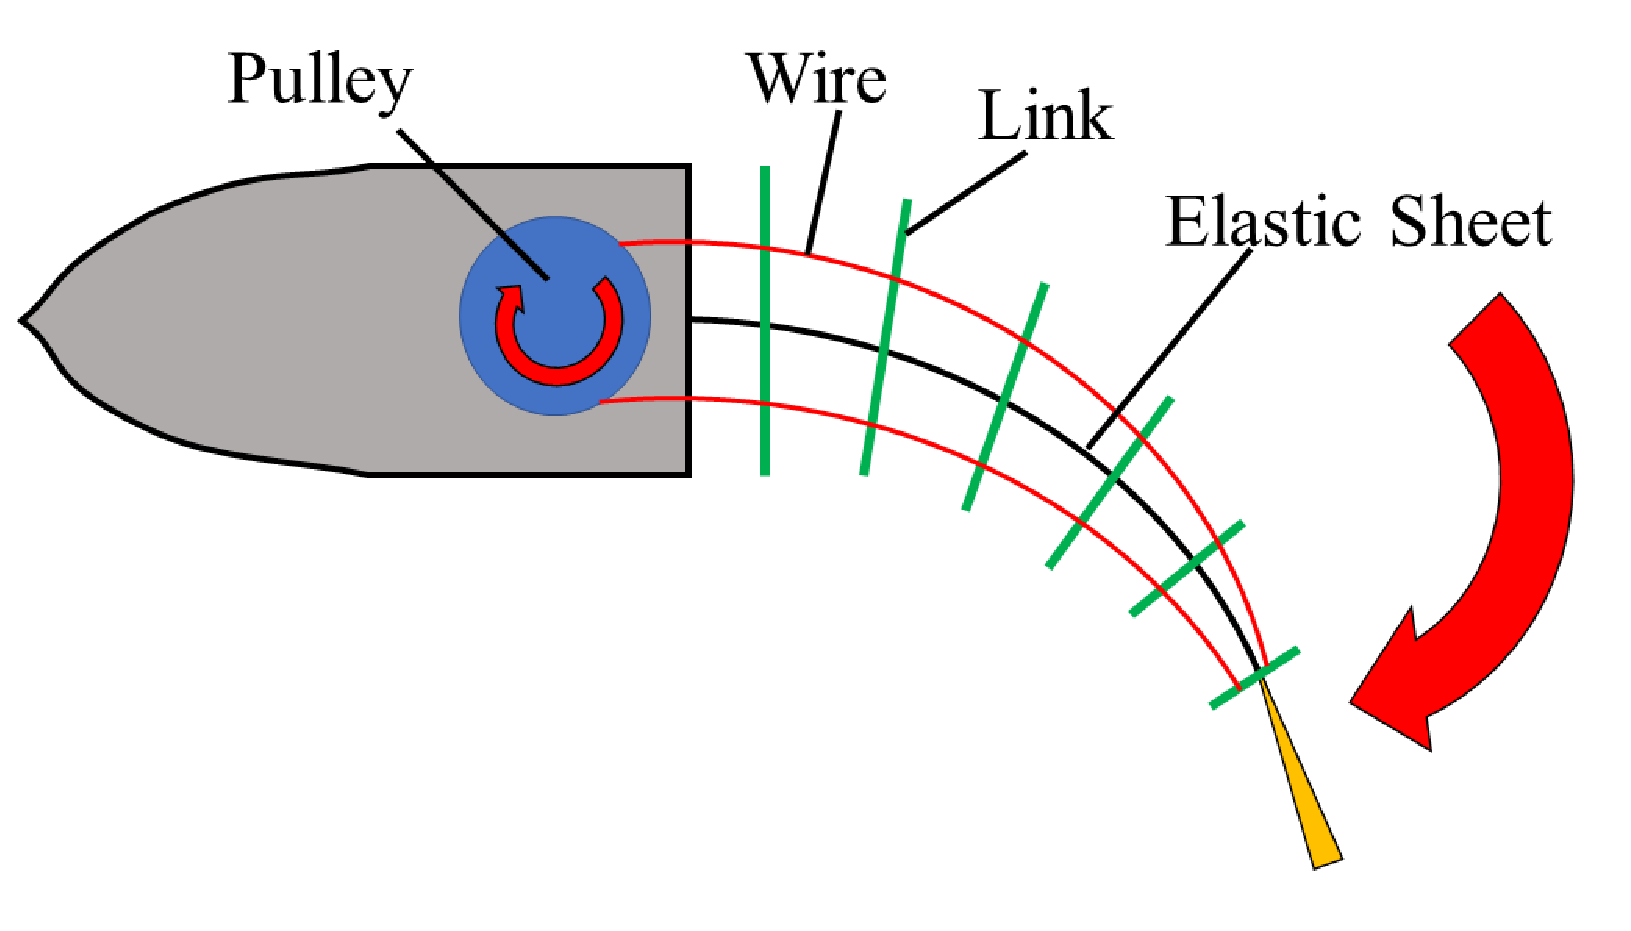
\includegraphics[width=0.6\linewidth]{chapters/picture/waiyakudou.eps}
   \caption{ワイヤ駆動のイメージ}
   \label{fig:waiyakudou}
\end{figure}

\subsection{試作機}
\subsubsection{試作機の作製}
まず,昨年度卒業研究を参考にして試作機を作製した.図\ref{fig:sisaku}に外観を,図\ref{fig:kouzou_sisaku}に構造を示す.全長は530 mm,重量は478 gである.試作機は頭部と胴体部の二つ
の部分で構成している.

頭部には制御回路とバッテリーを搭載しており,えらにあたる部分には防水仕様(IP67)の サーボモータ(Flash Hobby, M45CHW)を配置している.サーボモータは270°回転できるようになっている.
使用マイコンはM5Stamp Pico(M5Stack Technology 社),使用バッテリーはマイコン用の3.7 V,サーボモータ用の7.4 Vの二つのLi-ionバッテリーを使用している.そのため,頭部は防水が必要となり,
頭部の断面にOリングをはめ込むことによって防水を行っている.頭部はネジ穴が空いたものと,ナット用の穴が空いたものに分かれており,これらはM1.7ネジで固定される.
胴体部は骨格リンク(PLA樹脂)と弾性体(ポリプロピレン板,厚さ0.75 mm),尾びれ(TPU樹脂,厚さ2 mm)で構成されており,骨格リンクは図のように楕円形にして作製し,ワイヤ(ポリエステル製,0.40 mm)
を通す穴を空けている.

\begin{figure}[t]
    \centering
    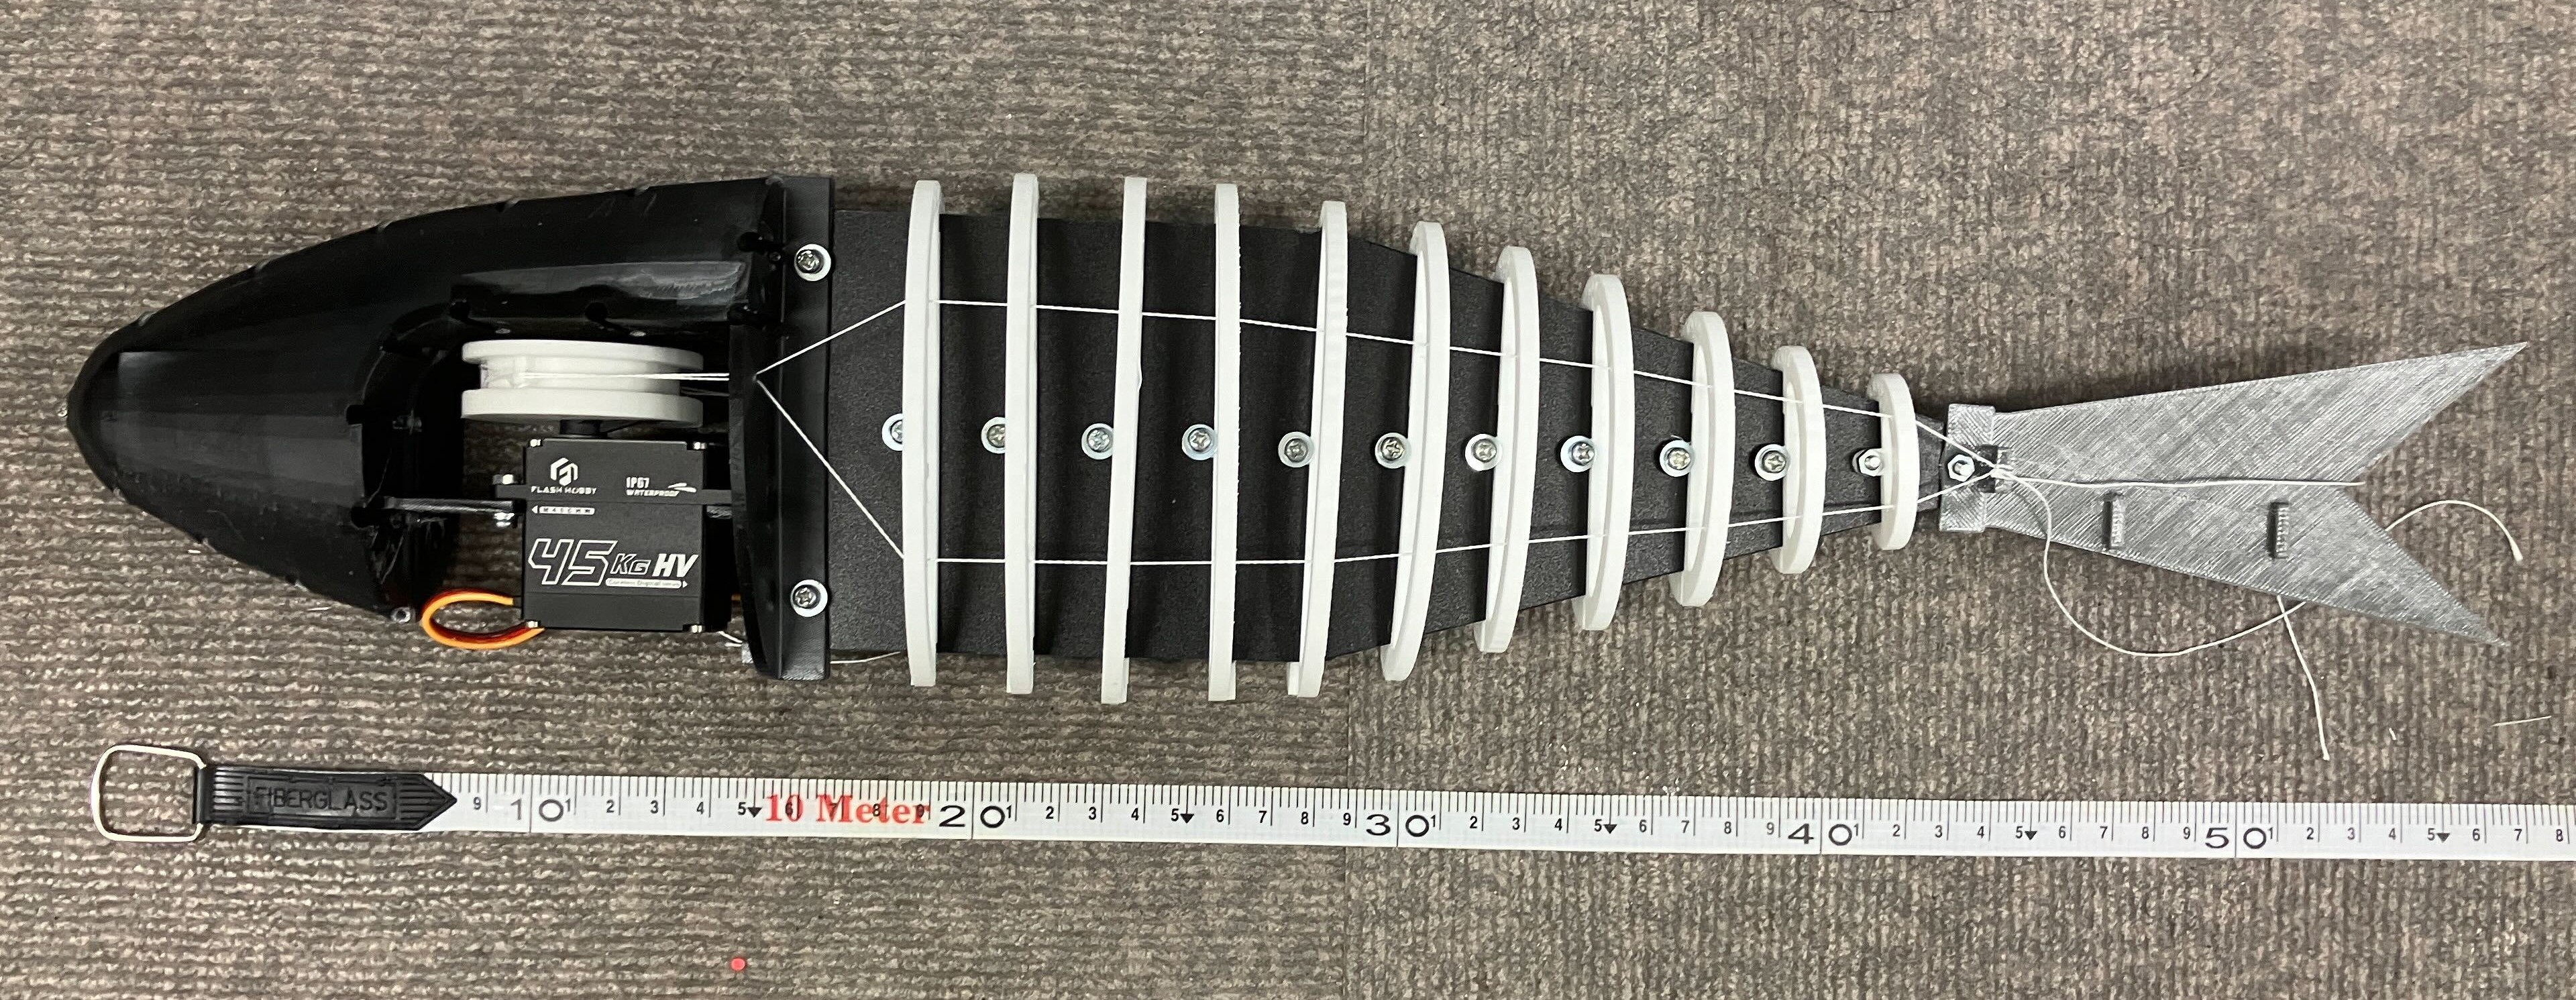
\includegraphics[width=0.80\linewidth]{chapters/picture/sisaku.jpg}
    \caption{試作機の外観}
    \label{fig:sisaku}
\end{figure}
\begin{figure}[t]
    \centering
    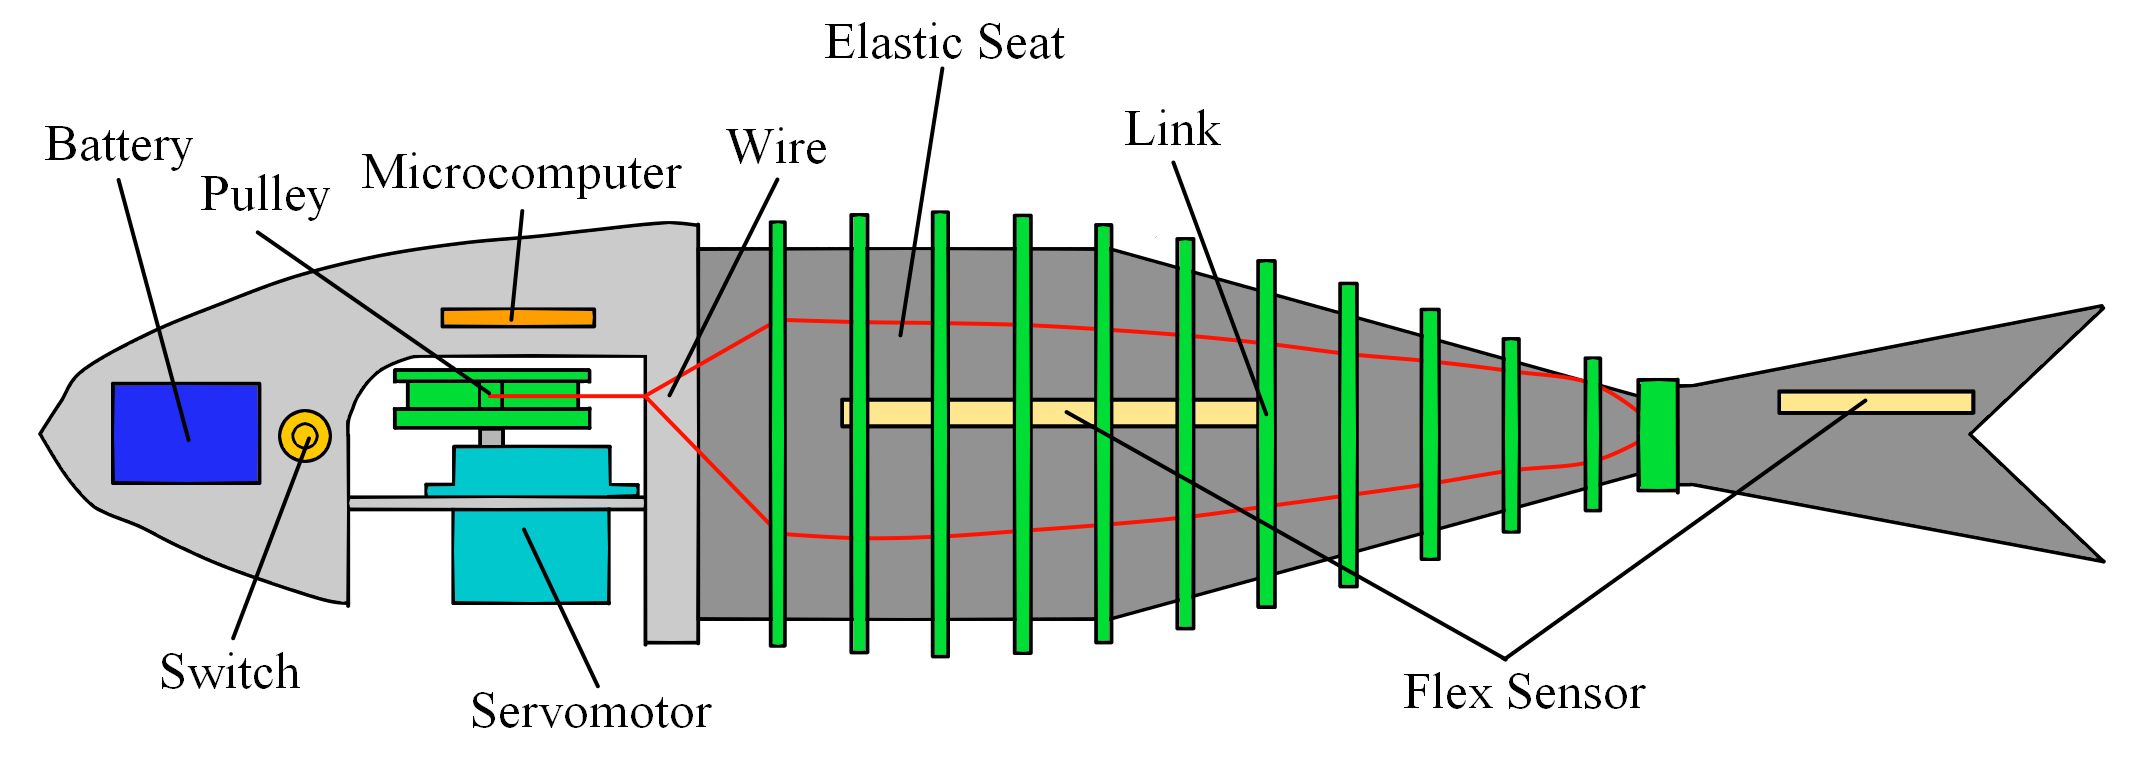
\includegraphics[width=0.80\linewidth]{chapters/picture/tentativeschematic.png}
    \caption{試作機の構造}
    \label{fig:kouzou_sisaku}
\end{figure}
\begin{figure}[t]
    \centering
     \begin{minipage}[b]{0.50\linewidth}
        \centering
        \setPicture{ring.jpg}
        \caption{頭部断面のようす}
        \label{fig:danmen}
     \end{minipage}
     \hspace{0.05\linewidth}
     \begin{minipage}[b]{0.25\linewidth}
        \centering
        \setPicture{jikkilink.png}
        \caption{骨格リンク}
        \label{fig:link_sen}
     \end{minipage}
\end{figure}

\subsubsection{防水テスト・遊泳テスト}
機体完成後,防水テストと遊泳テストを行った.まず防水テストは水没すると赤くなるシールを頭部内部に貼り,水深120 mmの水槽で2 分間沈める防水テストを7回行った.それぞれねじの締め具合や
頭部の歪みを直しながらテストをしたが,完全な防水はできず,7回目で頭部下方のみの浸水にとどまったのでこれで防水できていると判断した(図\ref{fig:bousuitest_sisaku}).
次に遊泳テストを行った.遊泳テストの様子を図\ref{fig:test_sisaku}に示す.

\begin{figure}[t]
    \centering
    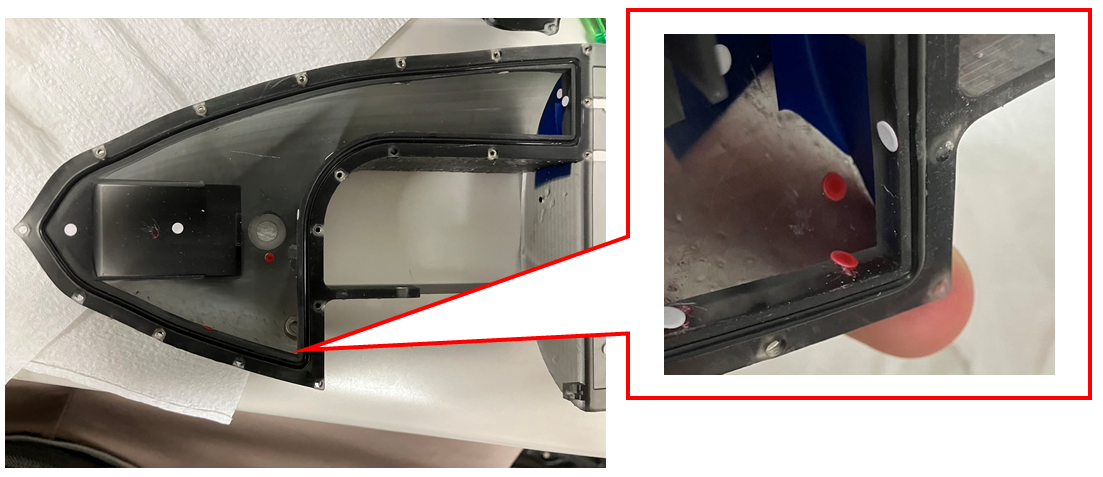
\includegraphics[width=0.80\linewidth]{chapters/picture/bousuitest.png}
    \caption{頭部下方浸水のようす}
    \label{fig:bousuitest_sisaku}
\end{figure}
\begin{figure}[t]
    \centering
    \setPicture{sisakuoyogu2.png}
    \caption{遊泳テストの様子}
    \label{fig:test_sisaku}
\end{figure}

\subsubsection{試作機から得られた知見}
試作機の作製・動作確認を通して得られた知見として,まず,頭部をネジとOリングを用いて防水する方法は完全な防水に至らないと考えられる.また,頭部を固定するネジが多いと,バッテリー交換が
しにくく,メンテナンス性が悪くなるということも分かった.以上のことから防水方法を変更し,メンテナンス性を向上させた頭部に改良することが必要だと考える.そこで防水を比較的容易な方法ででき,
完全防水可能な柔軟外皮を用いて頭部の防水を行うようにする.また,骨格リンクが胴体の形状をなしていることを生かし,骨格リンクをはめられるような溝を胴体外皮内部に作製することでリンクと
外皮の追従を行う.
% 必要に応じて章を増やす,またファイル名もsec2, sec3である必要はない
% このmain.texが置いてあるディレクトリ内にある「chapters」フォルダ以下に
% 自分がわかりやすい名前のtexファイルを作成し,\include{chapters/*****}で
% 呼び出せば良い
\newpage
\section{結言}
本研究では,魚らしいしなやかな動きを可能にするワイヤ駆動式の魚ロボットをベースにリンクに外皮を追従させ,尾びれのみならず
胴体部まで振って泳ぐことが可能なロボットの開発を行った.そして実験結果から

      % 結言
\newpage
\section{謝辞} % 謝辞
% できればbibtexを使ってください

\newpage
\section{参考文献}
\begin{thebibliography}{9}
    \bibitem{ichi}
    平田宏一, 春海一佳, 瀧本忠教, 田村兼吉, 牧野雅彦, 児玉良明, 冨田宏. 魚ロボットに関する基礎的研究. 海上技術安全研究所報告, Vol. 2, No. 3, pp. 281-307, 2003.
 
    \bibitem{ni}
    高田洋吾, 中西志允, 荒木良介, 脇坂知行. Piv 測定と3 次元数値解析による小型魚ロボット周りの水の流動状態と推進能力の検討(機械力学, 計測, 自動制御). 日本機械学会論文集C 編, Vol. 76, No. 763, pp. 665–672, 2010.

    \bibitem{san}
    高田洋吾, 中村毅志, 小山圭介, 田尻智紀. 色情報に基づく小型魚ロボットfocus の目標物追従制御. 日本機械学会論文集C 編, Vol. 78, No. 792, pp. 2924–2934, 2012.

    \bibitem{yon}
    中西大輔, 山根拓真, 末岡裕一郎, モータ・ワイヤ駆動併用型飛び移り座屈機構を用いた魚型ロボットの開発, ロボティクス・メカトロニクス講演会2020, 1P1-C04, 2020

    \bibitem{go}
    末岡裕一郎, 花原健太郎, 中西大輔, 大須賀公一. ワイヤ駆動の飛び移り座屈機構を搭載した魚型ロボットの大振幅遊泳. ロボティクス・メカトロニクス講演会講演概要集2020, 1P1–C05. 一般社団法人日本機械学会, 2020.

    \bibitem{roku}
    板垣達也, 中西大輔. しなやかな胴体を有する飛び移り座屈駆動式魚型ロボットの開発.ロボティクス・メカトロニクス講演会講演概要集2021, 2P3–H10. 一般社団法人日本機械学会, 2021.

    \bibitem{nana}
    中西大輔, 吉岡祐亮, ワイヤ駆動と連続飛び移り座屈機構を併用した魚型ロボットの開発, 第23回 公益社団法人 計測自動制御学会システムインテグレーション部門講演会, 1P3-H05, 2022.

    \bibitem{hachi}
    中西 大輔,高橋 海成,飛び移り座屈駆動式魚型ロボットによる旋回遊泳の実現, 第24回計測自動制御学会システムインテグレーション部門講演会(SI2023), 2C4-05, 2023.

    \bibitem{kyu}
    中西大輔, 石原康平, 柔軟外皮を有する飛び移り座屈駆動式魚型ロボットの開発. ロボティクス・メカトロニクス講演会2024, 2P2-B10, 2024.

    \bibitem{juu}
    神部勉, 魚の運動と渦. nagare, 1976, 8.3: 2-10.

    \bibitem{juuiti}
    朝日電装株式会社, "シール技術", 要素技術, \url{https://www.ad-asahidenso.co.jp/technology/water-proof_dust-proof/sealing/}, (参照 2024-12-13)

\end{thebibliography}


    % 参考文献

\end{document}
